%% Template.tex; Solar Physics
%% 
\documentclass[namedreferences]{SolarPhysics}
%
% spr-sola-addons available options:
%  natbib        -- For citations: redefine \cite commands
%  solaenum      -- makes enumerated list with italics-roman numerals and a single right-bracket
%  linksfromyear -- loads a natbib and puts a link on a year citation (hyperref must be loaded)
%  optionalrh    -- for optional running title/author
%
\usepackage[optionalrh,solaenum]{spr-sola-addons} % For Solar Physics 
%\usepackage{epsfig}                     % For eps figures, old commands
\usepackage{graphicx}                    % For eps figures, newer & more powerfull
%\usepackage{courier}                    % Change the \texttt command to courier style
%\usepackage{amssymb}                    % useful mathematical symbols
\usepackage{color}                       % For color text: \color command
\usepackage{url}                         % For breaking URLs easily trough lines
\def\UrlFont{\sf}                        % define the fonts for the URLs


%% Local definitions
%% please place your own definitions here and don't use \def but
%% \newcommand{}{} or 
%% \renewcommand{}{} if it is already defined in LaTeX



%%%%%%%%%%%%%%%%%%%%%%%%%%%%%%%%%%%%%%%%%%%%%%%%%%%%%%%%%%%%%%%%%%
\begin{document}

\begin{article}

\begin{opening}

\title{THE HELIO 100 CME CHALLENGE}

%%%%%%%%%%%%%%%%%%%%%%%%%%%%%%%%%%%%%%%%%%%%%%%%%%%
%% Authors Names
%
\author{J.~P.~\surname{Byrne}$^{1}$\sep
B.~\surname{Cecconi}$^{2}$\sep
D.~\surname{P\'erez-Su\'arez}$^{3}$\sep
E.~\surname{Carley}$^{3}$\sep
S.~A.~\surname{Maloney}$^{4}$\sep
G.~\surname{Pierantoni}$^{5}$\sep
N.~\surname{Bourrel}$^{6}$\sep
A.~\surname{Lynnyk}$^{6}$\sep
F.~\surname{Mayer}$^{7}$\sep
\& the HELIO team.
%        I.~\surname{}$^{2}$      
       }


%%%%%%%%%%%%%%%%%%%%%%%%%%%%%%%%%%%%%%%%%%%%%%%%%%%
%% Runningheads
%
%\runningauthor{}
%\runningtitle{}


%%%%%%%%%%%%%%%%%%%%%%%%%%%%%%%%%%%%%%%%%%%%%%%%%%%
%% Affilations 
%
  \institute{$^{1}$ Institute for Astronomy, University of Hawaii, Honolulu, USA.
                     email: \url{jbyrne@ifa.hawaii.edu} \\ 
              $^{2}$ LESIA, Observatoire de Paris, Meudon, France. \\
              $^{3}$ School of Physics, Trinity College Dublin, Dublin, Ireland. \\
              $^{4}$ Skytek Ltd., Dublin, Ireland. \\
              $^{5}$ School of Computer Science and Statistics, Trinity College Dublin,
Dublin, Ireland. \\
              $^{6}$ Research Institute in Astrophysics and Planetology (IRAP) -
CNRS/UPS, Toulouse, France. \\
              $^{7}$ Technische Universit�t Wien, Austria. \\
%                     email: \url{e.mail-c} \\
             }


%%%%%%%%%%%%%%%%%%%%%%%%%%%%%%%%%%%%%%%%%%%%%%%%%%%
%%% Abstract 
\begin{abstract}

Studying the propagation and impact of solar eruptive events and their various manifestations is of great importance for understanding and predicting space weather conditions in the heliosphere. The Heliophysics Integrated Observatory (HELIO) was generated out of a need to robustly link the detections of solar-driven events at different locations in space, via remote-sensing and in-situ instruments onboard various spacecrafts. Under development since 2009, HELIO is now at a stage of great scientific benefit for large-scale studies of solar and heliospheric phenomena, through the generation of workflows that use HELIO to access and cross-correlate event lists and their measured properties.

%Geomagnetic storms at Earth can cause adverse effects on global communication networks, satellite operations, and human space travel. This is of increased importance in the current era of complex global communication systems, space-based communication systems, human space travel, and especially their potentially adverse effects in the vicinity of the Earth.


The fourth HELIO coordinated data analysis workshop (HELIO CDAW-4) held in Trinity College Dublin in September 2012 outlined three challenges to be addressed by working groups comprising solar physicists and computer scientists. The challenges were titled: (1) ``Heliospheric variability over the solar cycle"; (2) ``The 100 CME challenge"; and (3) ``HELIO as a tool for space weather". In this paper we outline the success of challenge (2), that focused on using HELIO to study the origin, propagation and impacts of a large number of coronal mass ejections (CMEs) in the heliosphere. HELIO provides an interface that allows researchers to track active regions as they evolve and produce solar flares and CMEs. Once launched, CMEs can be tracked in coronagraph and heliospheric images. Their impacts throughout the heliosphere can then be measured using in-situ instruments from a number of spacecraft throughout the solar system. The aim of this challenge was to use HELIO to track a large number of CMEs that had an associated type II radio burst from their source region on the surface of the Sun, and possible flare occurrence, to their effects through interplanetary space. This was achieved through the generation of a workflow that accessed the corresponding event lists and used a ballistic CME propagation model to predict each event's arrival time at Earth and elsewhere in the solar system. This provides a timeframe for determining the in-situ parameters measured at the different spacecraft locations where a CME impact was detected, and thus allows us to combine the data across multiple spacecrafts on a per-event basis for comprehensive analysis of the physics of their propagation and evolution.


\end{abstract}



%%%%%%%%%%%%%%%%%%%%%%%%%%%%%%%%%%%%%%%%%%%%%%%%%%%
%% Keywords
%
%\keywords{}


\end{opening}
%-------------------------------------------------

%%%%%%%%%%%%%%%%%%%%%%%%%%%%%%%%%%%%%%%%%%%%%%%%%%%
%% Sections
%
% \section{}%\label{s:?} 
\section{Introduction}

\begin{figure} 
\centerline{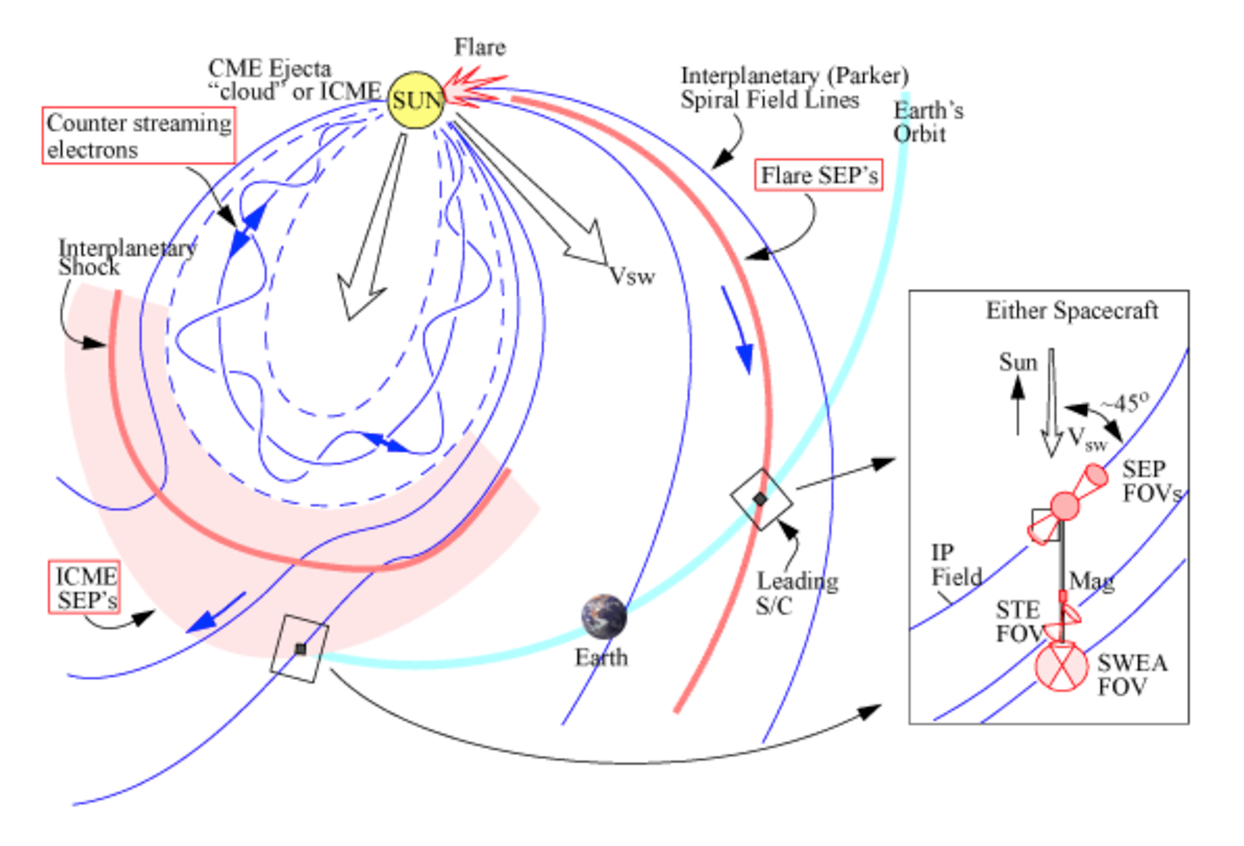
\includegraphics[width=\textwidth, clip=]{images/science_of_impact_c.pdf}}
\caption{}%\label{fig:?}
\end{figure}

\section{Building a workflow}

The challenge group began by choosing a \emph{test case} CME for tracking through the HELIO interface, and building a model workflow to be ultimately extended for a large scale study of many events. The CME chosen was a fast event associated with a flare and type II radio burst, as listed in the `Wind/WAVES type II bursts and CMEs list\footnote{http://cdaw.gsfc.nasa.gov/CME\_list/radio/waves\_type2.html}. The radio burst was detected at 04:20~UT on 11~April~2004, with an associated NOAA C\,9.6 flare at disk location S\,14\,W\,47, and CME observed  in LASCO at 04:30~UT with central position angle 203$^{\circ}$, angular width 314$^{\circ}$, and speed 1645\,km\,s$^{-1}$.

The workflow was built in the following manner, with the \emph{test case} inputs/outputs as specified:

% 2004/04/11 04:20 04/11 05:35 14000   500   S14W47 10588 C9.6   04/11 04:30  203  314 1645   PHTX

\begin{enumerate}
\setlength{\itemsep}{6pt}

\item A time interval is specified and input to the `Wind/WAVES type II bursts and CMEs list\footnotemark[\value{footnote}] to retrieve a list of events within the given time-range of interest.

\emph{Time range: 2004/04/01~00:00:00 -- 2004/04/30~~00:00:00}

\item The list of candidate events were ranked in order of decreasing CME speed, with the intent that the top 100 across a large time-range be chosen for the purposes of this challenge. (The single fastest event in the \emph{test case} sample was chosen, as described above.)

\begin{tabular}{l l}
\emph{Type II burst} & \emph{Time range: 2004/04/11~04:20\,--\,05:35} \\
& \emph{Frequency: 14000\,--\,500~kHz} \\
\emph{Flare} & \emph{Location: S14W47} \\
& \emph{NOAA: 10588} \\
& \emph{Class: C9.6} \\
\emph{CME} & \emph{Start time: 2004/04/11~04:30} \\
& \emph{Central position angle: 203$^{\circ}$} \\
& \emph{Angular width: 314$^{\circ}$} \\
& \emph{Speed: 1645~km~s$^{-1}$} \\
\end{tabular}


\item The GOES Soft X-ray Flare List\footnote{http://www.ngdc.noaa.gov/stp/solar/solarflares.html} was then inspected for any associated flaring activity of the relevant class, within a specified window of $\pm$1~hour on the start time of the type II burst, to obtain the catalogued source longitude on disk.

\emph{Time range: 2004/04/11~03:20\,--\,05:20}

\emph{Peak flare time (t$_{start}$): 04:19}

\emph{Longitude ($\lambda_{lon}$): 46$^{\circ}$}

\item The SOHO LASCO CME Catalogue\footnote{http://cdaw.gsfc.nasa.gov/CME\_list/} is inspected in order to associate CME parameters from the relevant detection in the time range of the type II burst. In this case the necessary parameters are the CME initial and final speeds, and angular width. The choice of catalogue can be changed, for example to call one of the automated CME catalogues such as CACTus.

\begin{tabular}{l l}
\emph{v$_{init}$\,:} & \emph{1953$~km~s^{-1}$} \\
\emph{v$_{final}$\,:} & \emph{1340$~km~s^{-1}$} \\
\emph{$\theta_{width}$\,:} & \emph{314$^{\circ}$} \\
\end{tabular}

\item The CME speed is determined as $v_{cme} = v_{final} \,\pm\, \sigma_v$ where an initial estimate of the uncertainty on the CME speed is calculated as $\sigma_v=\frac{\left|v_{final}-v_{init}\right|}{2}$. A clause is put on the angular width that if it is greater than $180^{\circ}$, i.e., a halo CME where $\theta_{width}>180^{\circ}$, its true width is calculated as half the plane-of-sky width $\theta_{cme}=\theta_{width}/2$.

\begin{tabular}{l l}
\emph{v$_{cme}$\,:} & \emph{1340 $\pm$ 306.5$~km~s^{-1}$} \\
\emph{$\theta_{cme}$\,:} & \emph{157$^{\circ}$} \\
\end{tabular}

\item The HELIO ballistic CME model is run with the following input parameters: CME start time from the peak time of the associated flare $t_{start}$; trajectory from the associated flare longitude $\lambda_{lon}$; speed $v_{cme}$, and angular width $\theta_{cme}$.

%\begin{tabular}{l l}
%\emph{t$_{start}$}\,: & \emph{2004/04/11\,T\,04:19} \\
%\emph{$\lambda_{lon}$}\,: & \emph{46$^{\circ}$} \\
%\emph{

\item From the ballistic CME model, an expected timeframe of arrival at the L1 point (the first Lagrangian point, near Earth) is determined. If an event is not deemed Earth-directed it is flagged as so. The in-situ data from the ACE spacecraft is queried via the Automated Multi Dataset Analysis web service\footnote{http://manunja.cesr.fr/Amda-Helio/}, and an average speed of the solar wind $\bar{v}_{sw}$ during this timeframe is calculated. 

\begin{tabular}{l l}
\emph{L1 timeframe:} & \emph{2004/04/12~05:57:54 -- 21:10:41} \\
\emph{$\bar{v}_{sw}$\,:} & \emph{442.33$~km~s^{-1}$} \\
\end{tabular}


\item From the average solar wind speed, a new velocity of the CME is calculated to essentially account somewhat for the influence of drag. The average solar wind speed is used to modify the input CME speed by lowering the uncertainty interval to match it as the lower bound (or raise it to the upper bound as the case may be, though unlikely for these candidate 100 fastest CMEs chosen). While the upper bound is kept fixed, the modified CME speed between the bounds is calculated as $v'_{cme} = \frac{1}{2} \left( \bar{v}_{sw} + \frac{v_{final}+v_{init}}{2} \right)$ with new uncertainty $\sigma'_v = \frac{1}{2}\left(\sigma_v +v_{final}- \bar{v}_{sw}\right)$. These are used to rerun the ballistic CME propagation model.

\begin{tabular}{l l}
\emph{$v'_{cme}$\,:} & \emph{1044 $\pm$ 602$~km~s^{-1}$} \\
\end{tabular}

\item The predicted impact timeframes of the CME at the relevant locations throughout the heliosphere are output from the workflow, e.g., in this case Mercury, Earth, and Voyager 1 \& 2 at the edge of the heliosphere. 

\begin{tabular}{l l}
\emph{Mercury arrival timeframe:} & \emph{2004/04/11~16:04:54 -- 2004/04/13~00:06:36} \\
\emph{Earth arrival timeframe:} & \emph{2004/04/12~05:57:54 -- 2004/04/15~03:47:20} \\
\emph{Voyager\,2 arrival timeframe:} & \emph{2004/06/28~00:00:00 -- 2005/02/02~00:00:00} \\
\emph{Voyager\,1 arrival timeframe:} & \emph{2004/07/18~00:00:00 -- 2005/02/05~00:00:00} \\
\end{tabular}

\end{enumerate}

\begin{figure} 
\centerline{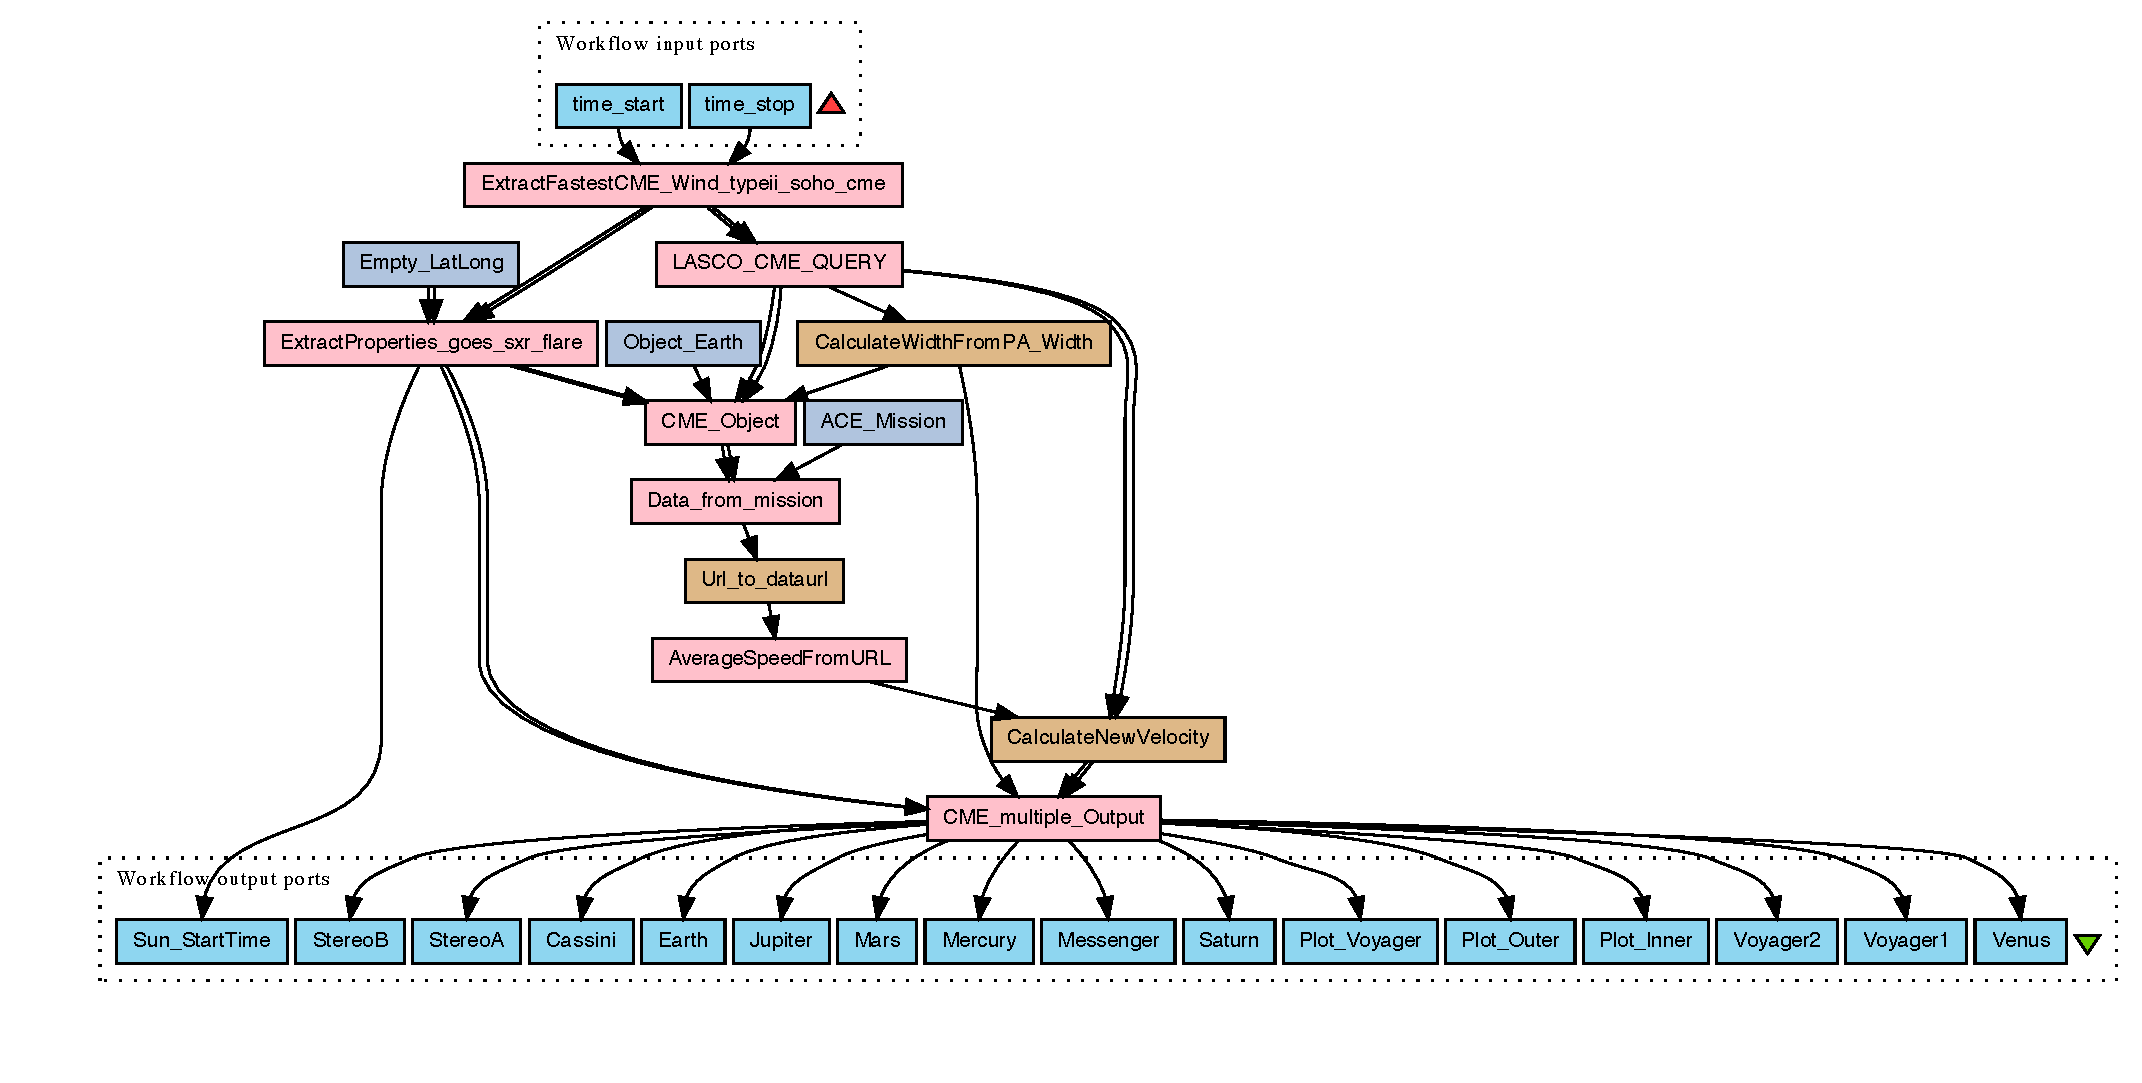
\includegraphics[width=\textwidth, clip=]{images/workflow.pdf}}
\caption{}%\label{fig:?}
\end{figure}




%% Figure 
%
% \begin{figure} 
% \centerline{\includegraphics[width=0.5\textwidth,clip=]{<fig.eps>}}
% \caption{}%\label{fig:?}
% \end{figure}



%% Table
%
% \begin{table}
% \caption{}%\label{tbl:?}
% \begin{tabular}{}     
% \hline
% \multicolumn{2}{c}{<>}
% <data>
% \hline
% \end{tabular}
% \end{table}
  

%%%%%%%%%%%%%%%%%%%%%%%%%%%%%%%%%%%%%%%%%%%%%%%%%%%%%%%%%%%%%%%%%%%%%%%%%%%
%% Appendix
%
% \appendix   



%%%%%%%%%%%%%%%%%%%%%%%%%%%%%%%%%%%%%%%%%%%%%%%%%%%%%%%%%%%%%%%%%%%%%%%%%%%
%% Acknowledgements
%
% \begin{acks}
%
% \end{acks}


%%% %%%%%%%%%%%%%%%%%%%%%%%%%%%%%%%%%%%%%%%%%%%%%%%%%%%%%%%%%%%
%% Bibliography
%
% Using BibTeX
%
%\bibliographystyle{spr-mp-sola}
\bibliographystyle{spr-mp-sola-cnd} %% Alternative style: no title, no concluding page
\bibliography{references.bib}  
%
% Without BibTeX 
% \begin{thebibliography}{}
% \bibitem[\protect\citeauthoryear{Author}{Year}]{key}
%   <bibliographical entry>
%
% \bibitem[\protect\citeauthoryear{}{}]{}
%   
%  
% \end{thebibliography}

\end{article} 
\end{document}
